\documentclass{article}
\usepackage{amsmath}
\usepackage{graphicx}

\title{Solution for Exercise 7 List 1}
\author{Krzysztof Tałałaj}
\date{\today}
\begin{document}
    \maketitle
    \section{Probability of insertion failure in DHT}

    Assuming that the hash functions used are good quality and produce uniformly distributed hash values, the probability that a specific address is already occupied is $\frac{1}{2^k}$, moreover knowing that there are $n$ files already inserted, the probability of occupation is approximately:
    $$P(a_i\text{ occupied}) \approx n \cdot \frac{1}{2^k} = \frac{n}{2^k}$$
    The probability  of failure to insert a new file $F$ at either address $a_1$ or $a_2$ is:
    \begin{gather}
        \nonumber P(\text{failure to insert F}) = P(a_1 \text{ and } a_2 \text{ occupied}) = \\
        = P(a_1 \text{ occupied}) \cdot P(a_2 \text{ occupied } | a_1 \text{    occupied})
    \end{gather}
    Since the addresses are chosen independently with the same probability, the conditional probability (1) that $a_2$ is occupied knowing that $a_1$ is occupied is also approximately $\frac{n}{2^k}$. So, the probability of failure to insert $F$ is:
    \begin{equation}
        P_{failure} \approx \left(\frac{n}{2^k}\right)^2
    \end{equation}

    \section{Example of Cuckoo filter insertion collision}

    With the DHT structure, when there is a collision during insertion, the item is simply not inserted. This can lead to a high probability of insertion failure, as shown in Section 1, especially when the table becomes more crowded. The Cuckoo filter attempts to resolve collisions by performing relocations of data.

    Figure 1 on the next page shows the example of inserting a new item x into occupied space. There could occur a situation, when we encounter infinite loop (when we once again try to relocate x into same place, because of relocation chain), we can then just rehash algorithm, meaning f.ex. changing the iv in used hashing functions or just changing them in any way. Handling the collisions in such way allows handling the insertion collisions to be amortized and still takes estimated O(1) complexity.

    \clearpage
    \begin{figure}[ht]
        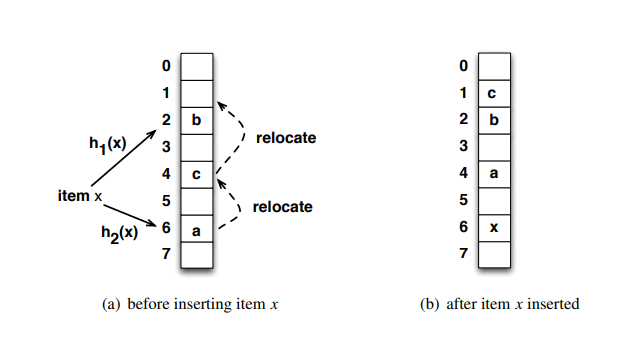
\includegraphics[width=.9\textwidth]{./cockoo.png}
        \caption{Collision while inserting x and rellocation process.}
    \end{figure}

    \section{Cuckoo improvement on DHT}

    One can try to calculate the new probability of insertion failure, but it would require some strict probability calculations, without them we can estimate it's value $p_{failure}^{cuckoo}$ to be somehow dependant on the $p_{failure}$ (2) and on the chosen limit of relocations $q$ done before assuming failure, and we can assume, because of added functionality, that it is more unlikely to fail than standard DHT.
    $$p_{failure}^{cuckoo}(q) << p_{failure}$$
    The intuition is that the longer relocation chain we allow - the probability shrinks rapidly. Chaining means, that we would have to find $q$ collisions in series, with the view of recursion, each position that we consider in a chain of depth $q$, would need a separate collision $2^q-\delta$ times. Knowing that probability of one is small, the  series is even more unlikely the longer series we consider.
    $$p_{failure}^{cuckoo}(q) \approx (p_{failure})^{2^q-\delta} = \left[\left(\frac{n}{2^k}\right)^2\right]^{2^q-\delta}$$
    The Cuckoo filter addition to DHT structure attempts to resolve collisions by evicting previously inserted items and moving them to their alternative positions. This allows the new item to take their place, resulting in a higher probability of successful insertion. The Cuckoo filter allows for a higher load factor and better space utilization, resulting in a smaller memory footprint for the filter. The constant-time insertions, lookups and deletions of the Cuckoo filter also make it an efficient data structure.

    Overall, the Cuckoo filter's ability to handle insertion failures and its efficiency in space and time can make it a very useful choice for applications such as network routers and web caches.

    \section{Points: 5/5}

\end{document}